\documentclass[11pt,a4paper,titlepage]{article}
\usepackage[a4paper]{geometry}
\usepackage[utf8]{inputenc}
\usepackage[english, portuges]{babel}

\selectlanguage{portuges}

\usepackage{lipsum}

\usepackage{amsmath, amssymb, amsfonts, amsthm, fouriernc, mathtools}
% mathtools for: Aboxed (put box on last equation in align envirenment)
\usepackage{microtype} %improves the spacing between words and letters

\usepackage{graphicx}
\usepackage{epsfig}
\usepackage{epstopdf}


%%%%%%%%%%%%%%%%%%%%%%%%%%%%%%%%%%%%%%%%%%%%%%%%%%
%% COLOR DEFINITIONS
%%%%%%%%%%%%%%%%%%%%%%%%%%%%%%%%%%%%%%%%%%%%%%%%%%
\usepackage[svgnames]{xcolor} % Enabling mixing colors and color's call by 'svgnames'
%%%%%%%%%%%%%%%%%%%%%%%%%%%%%%%%%%%%%%%%%%%%%%%%%%
\definecolor{MyColor1}{rgb}{0,0,0} %mix personal color
\newcommand{\textb}{\color{Black} \usefont{OT1}{lmss}{m}{n}}
%\newcommand{\textb}{\color{MyColor1} \usefont{OT1}{lmss}{m}{n}}
%\newcommand{\textb}{\color{MyColor1} \usefont{OT1}{lmss}{b}{n}}
\newcommand{\red}{\color{Black} \usefont{OT1}{lmss}{m}{n}}
\newcommand{\green}{\color{Black} \usefont{OT1}{lmss}{m}{n}}
%%%%%%%%%%%%%%%%%%%%%%%%%%%%%%%%%%%%%%%%%%%%%%%%%%


%%%%%%%%%%%%%%%%%%%%%%%%%%%%%%%%%%%%%%%%%%%%%%%%%%
%% FONTS AND COLORS
%%%%%%%%%%%%%%%%%%%%%%%%%%%%%%%%%%%%%%%%%%%%%%%%%%
%    SECTIONS
%%%%%%%%%%%%%%%%%%%%%%%%%%%%%%%%%%%%%%%%%%%%%%%%%%
\usepackage{titlesec}
\usepackage{sectsty}
%%%%%%%%%%%%%%%%%%%%%%%%
%set section/subsections HEADINGS font and color
\sectionfont{\color{Black}}  % sets colour of sections
\subsectionfont{\color{Black}}  % sets colour of sections

%set section enumerator to arabic number (see footnotes markings alternatives)
\renewcommand\thesection{\arabic{section}.} %define sections numbering
\renewcommand\thesubsection{\thesection\arabic{subsection}} %subsec.num.

%define new section style
\newcommand{\mysection}{
\titleformat{\section} [runin] {\usefont{OT1}{lmss}{b}{n}\color{Black}} 
{\thesection} {3pt} {} } 

%%%%%%%%%%%%%%%%%%%%%%%%%%%%%%%%%%%%%%%%%%%%%%%%%%
%		CAPTIONS
%%%%%%%%%%%%%%%%%%%%%%%%%%%%%%%%%%%%%%%%%%%%%%%%%%
\usepackage{caption}
\usepackage{subcaption}
%%%%%%%%%%%%%%%%%%%%%%%%
\captionsetup[figure]{labelfont={color=Black}}

%%%%%%%%%%%%%%%%%%%%%%%%%%%%%%%%%%%%%%%%%%%%%%%%%%
%		!!!EQUATION (ARRAY) --> USING ALIGN INSTEAD
%%%%%%%%%%%%%%%%%%%%%%%%%%%%%%%%%%%%%%%%%%%%%%%%%%
%using amsmath package to redefine eq. numeration (1.1, 1.2, ...) 
%%%%%%%%%%%%%%%%%%%%%%%%
\renewcommand{\theequation}{\thesection\arabic{equation}}

%set box background to grey in align environment 
\usepackage{etoolbox}% http://ctan.org/pkg/etoolbox
\makeatletter
\patchcmd{\@Aboxed}{\boxed{#1#2}}{\colorbox{black!15}{$#1#2$}}{}{}%
\patchcmd{\@boxed}{\boxed{#1#2}}{\colorbox{black!15}{$#1#2$}}{}{}%
\makeatother
%%%%%%%%%%%%%%%%%%%%%%%%%%%%%%%%%%%%%%%%%%%%%%%%%%




%%%%%%%%%%%%%%%%%%%%%%%%%%%%%%%%%%%%%%%%%%%%%%%%%%
%% DESIGN CIRCUITS
%%%%%%%%%%%%%%%%%%%%%%%%%%%%%%%%%%%%%%%%%%%%%%%%%%
\usepackage[siunitx, american, smartlabels, cute inductors, europeanvoltages]{circuitikz}
%%%%%%%%%%%%%%%%%%%%%%%%%%%%%%%%%%%%%%%%%%%%%%%%%%



\makeatletter
\let\reftagform@=\tagform@
\def\tagform@#1{\maketag@@@{(\ignorespaces\unskip\@@italiccorr)}}
\renewcommand{\eqref}[1]{\textup{\reftagform@{\ref{#1}}}}
\makeatother
\usepackage{hyperref}
\hypersetup{colorlinks=false}

%%%%%%%%%%%%%%%%%%%%%%%%%%%%%%%%%%%%%%%%%%%%%%%%%%
%% PREPARE TITLE
%%%%%%%%%%%%%%%%%%%%%%%%%%%%%%%%%%%%%%%%%%%%%%%%%%
\title{Documentação da Arquitetura do Projeto \\
MAC0218 - Técnicas de Programação II\\
Última Entrega}
\author{Mateus Agostinho dos Anjos - 9298191\\Nícolas Nogueira Lopes da Silva - 9277541\\Victor Domiciano Mendonça - 8641963}
\date{30 de junho de 2018}
%%%%%%%%%%%%%%%%%%%%%%%%%%%%%%%%%%%%%%%%%%%%%%%%%%



\begin{document}
\maketitle

\tableofcontents

\pagebreak

\section{Introdução}
Esta documentação fornece uma visão geral da arquitetura do sistema a ser implementado. Com a proposta e escopo da aplicação, requisitos funcionais e não-funcionais, além de diagramas de casos de uso e do modelo de banco de dados implementado.

\section{Projeto}
\subsection{Propósito e Escopo}
O propósito desta aplicação é permitir com que usuários possam interagir com o envio de mensagens instantâneas como uma aplicação de chat. Os usuários vão poder se comunicar usuário para usuário, de forma semelhante a de um Web Chat, onde existe uma lista de usuários públicas e eles conversam entre si. A aplicação será escrita em Ruby com utilização do Rails e todos os aspectos da aplicação serão desenvolvidos e testados.
\subsection{Dependências do sistema}
\begin{itemize}
\item Ruby v. 2.5.0
\item Rails v. 5.1.4
\item sqlite3
\end{itemize}
\subsection{Requisitos funcionais}
\begin{itemize}
\item Uma conta de usuário possui obrigatóriamente um login, um email e uma senha vinculados.
\item Cada usuário possui uma conta com: um perfil contendo seu login e seu email, possuindo acesso à lista de usuários pública para conversa. 
\item Um perfil de usuário possui obrigatoriamente um apelido único. Pode possuir uma imagem vinculada com o email através do gravatar.
\item Os perfis de usuários podem ser encontrados na lista pública de usuários.
\item Usuários podem trocar mensagens com outros usuários através da lista de usuários.
\item O aplicativo deve permitir o envio de mensagens de um usuário para um usuário que não esteja conectado no momento, a mensagem enviada deve aparecer para o destinatário quando este logar no sistema.
\end{itemize}
\subsection{Requisitos não funcionais}
\begin{itemize}
\item O aplicativo precisa possuir uma interface amigável ao usuário, como todo bom chat deve possuir.
\end{itemize}

\section{Banco de Dados}

O modelo de banco de dados foi implementado, a base de usuários está funcionando, não implementamos a gerência de contatos e grupos originalmente pensada.
\begin{figure}[!ht]
	\centering
	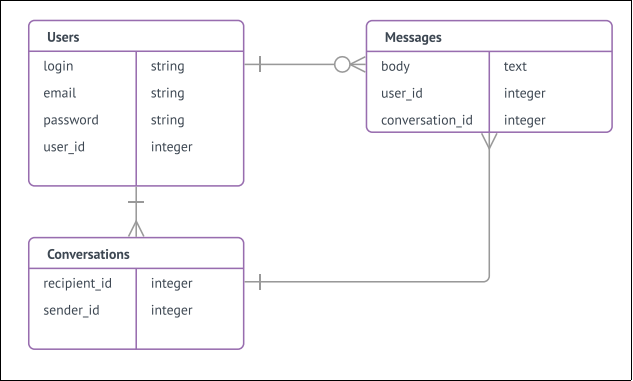
\includegraphics[scale=0.7]{img/db.png}
	\caption{Diagrama Entidade-Relacionamento do Banco de Dados}
\end{figure}
\pagebreak
\section{Diagrama de Casos de Uso Antigo}
Do projeto original, planejávamos fazer o sistema seguindo esses casos de uso.
\begin{figure}[!ht]
	\centering
	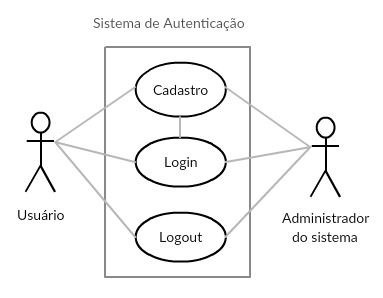
\includegraphics[scale=0.8]{img/casosautenticacao.png}
	\caption{Diagrama de Casos de Uso do Sistema de Autenticação.}
\end{figure}
\begin{figure}[!htb]
	\centering
	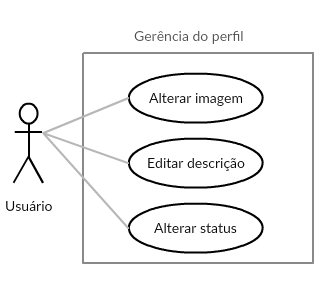
\includegraphics[scale=0.8]{img/casosperfil.png}
	\caption{Diagrama de Casos de Uso da Gerência de Perfil.}
\end{figure}
\begin{figure}[!htb]
	\centering
	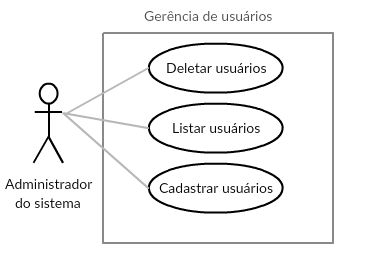
\includegraphics[scale=0.8]{img/casosusuarios.png}
	\caption{Diagrama de Casos de Uso da Gerência de Usuários.}
\end{figure}
\begin{figure}[!htb]
	\centering
	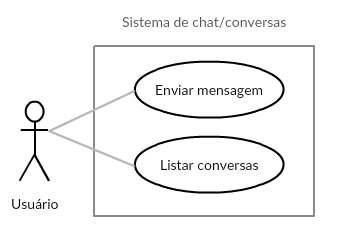
\includegraphics[scale=0.8]{img/casoschat.png}
	\caption{Diagrama de Casos de Uso do Sistema de Chat/Conversas.}
\end{figure}
\pagebreak
\begin{figure}[!htb]
	\centering
	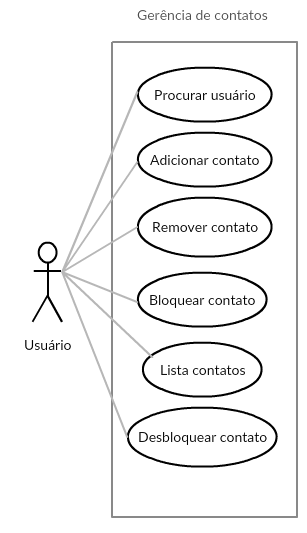
\includegraphics[scale=0.8]{img/casoscontatos.png}
	\caption{Diagrama de Casos de Uso da Gerência de Contatos.}
\end{figure}
\pagebreak
\begin{figure}[!htb]
	\centering
	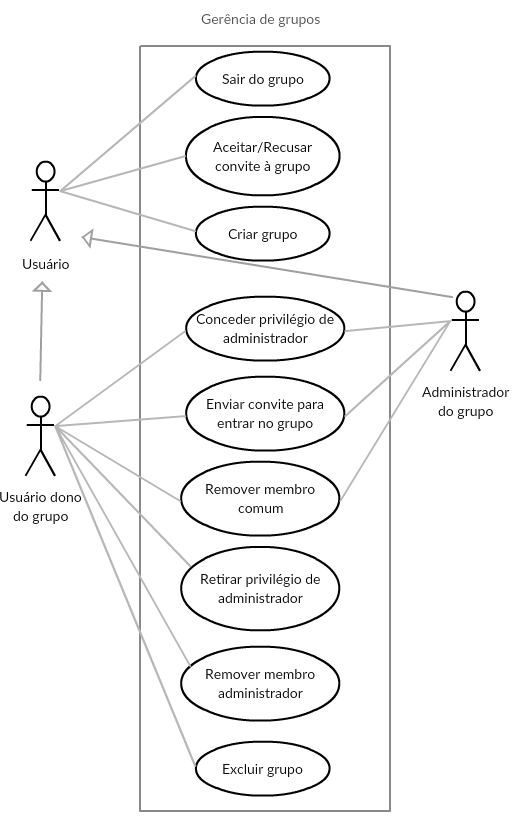
\includegraphics[scale=0.8]{img/casosgrupos.png}
	\caption{Diagrama de Casos de Uso da Gerência de Grupos.}
\end{figure}
\end{document}
